% Chapter 1

\chapter{Implementare} % Write in your own chapter title
\label{Capitolul4}
\lhead{Capitolul 4. \emph{Implementare}} % Write in your own chapter title to set the page header

\section{Generatorul de semnal BK4070}

Modelul BK4070 este o surs\u{a} de semnal capabil\u{a} s\u{a} genereze o varietate de forme de und\u{a}. Panoul frontal prezint\u{a} doi conectori de ie\c{s}ire. Conectorul SIG Out este principala ie\c{s}ire de semnal. Conectorul SYNC Out este o ie\c{s}ire de semnal dreptunghiular compatibil TTL/CMOS. Acest semnal este de +5V \c{s}i este util pentru comanda diverselor circuite digitale.

Unitatea dispune de asemenea de un conector RS-232 pe panoul din spate. Acesta permite utilizatorului s\u{a} controleze de la distan\c{t}a generatorul, utiliz\^{a}nd caractere ASCII. Nu sunt necesare componente sau protocoale speciale; orice terminal sau port serial de calculator pot fi utilizate. Viteza este reglabil\u{a}, p\^{a}n\u{a} la 115.2 Kbps. 

\section{Comenzile de control la distan\c{t}\u{a}}
Diagrama de mai jos prezint\u{a} tastele de pe panoul frontal \c{s}i codurile ASCII asociate lor. Trimiterea acestor caractere la BK4070 are acela\c{s}i efect ca \c{s}i ap\u{a}sarea butonului de pe panoul frontal.
\begin{figure}[!htb]
	\centering
	\includegraphics[scale=0.4]{panoufrontal.jpg}
	\caption{Tastele \c{s}i caracterele ASCII echivalente de pe panoul frontal}
	\label{panoufrontal}
\end{figure}

\^{I}n plus fa\c{t}\u{a} de comenzile \^{i}n caractere ASCII, sunt disponibile comenzi suplimentare pentru opera\c{t}iuni de control de la distan\c{t}\u{a}. Acestea sunt:
\begin{itemize}
	\item A - reseteaz\u{a} aparatul la modul semnal sinusoidal;
	\item V - furnizeaz\u{a} versiunile hardware \c{s}i software;
	\item K1,0 - Activeaz\u{a}, Dezactiveaz\u{a} tastele de pe panoul frontal;
	\item E1,0 - Activeaz\u{a}, Dezactiveaz\u{a} transmiterea c\u{a}tre terminal a textului de pe LCD;
	\item F0-9 - Mut\u{a} cursorul la c\^{a}mpurile 0-9;
	\item ? sau H - afi\c{s}eaz\u{a} meniul Help;
	\item \textasciicircum E - returneaz\u{a} \textasciicircum C.
\end{itemize}

Exemplu:
\begin{verbatim}
B F1 3.141Z N 2.3Z F0
\end{verbatim}
\begin{itemize}
	\item B - seteaz\u{a} aparatul \^{i}n modul semnal sinusoidal;
	\item F1 - mut\u{a} cursorul la c\^{a}mpul 1;
	\item 3.141Z - valoarea frecven\c{t}ei de 3.141 MHz;
	\item N - mut\u{a} cursorul la urm\u{a}torul c\^{a}mp;
	\item 2.3Z - valoarea de +2.3 dBm;
	\item F0 - mut\u{a} cursorul la c\^{a}mpul 0.
\end{itemize}

\section{Modul Basic Sinewave}
Acest mod genereaz\u{a} semnal sinusoidal de o anumit\u{a} frecven\c{t}\u{a}. Cei doi parametri necesari sunt Frecven\c{t}a \c{s}i Nivelul.

Pentru generarea unui semnal sinusoidal de 5000 KHz, 4 Vp-p, comanda va fi:

\begin{verbatim}B F1 5000X F2 4Y \end{verbatim}

Comenzile SCPI echivalente sunt:
\begin{verbatim}
SOURce:FREQuency 5000
SOURce:VOLTage 4
FUNCtion SINusoid
\end{verbatim}

\section{Modul Internal AM}
Acest mod genereaz\u{a} semnal modulat \^{i}n amplitudine folosindu-se un semnal sinusoidal generat intern ca semnal modulator. Parametrii necesari sunt Frecven\c{t}a de modulare, Procentul modula\c{t}iei, Frecven\c{t}a purt\u{a}toarei \c{s}i Nivelul PEP.

Exemplu:
\begin{verbatim}
M1 1 F1 4000X F2 40Z F3 5000X F4 3Y
\end{verbatim}

Echivalentul SCPI:
\begin{verbatim}
SOURce:FREQuency 5000
SOURce:VOLTage 3
SOURce:AM:SOURce INTernal
SOURce:AM:DEPTh 40
SOURce:AM:INTernal:FREQuency 4000
SOURce:AM:STATe ON
\end{verbatim}

\section{Modul External AM}
Acest mod genereaz\u{a} semnal modulat \^{i}n amplitudine folosindu-se ca semnal modulator un semnal exterior. Parametrii necesari sunt Input Gain, Frecven\c{t}a purt\u{a}toarei, Nivel PEP.

Exemplu:
\begin{verbatim}
M1 2 F1 0Z F2 5000X F3 3Y
\end{verbatim}

Exhivalentul SCPI:
\begin{verbatim}
SOURce:FREQuency 5000
SOURce:VOLTage 3
SOURce:AM:SOURce EXTernal
SOURce:AM:STATe ON
\end{verbatim}

\section{Modul Internal FM}
Acest mod genereaz\u{a} semnal modulat \^{i}n frecven\c{t}\u{a}, folosindu-se de un semnal generat intern. Parametrii necesari sunt Frecven\c{t}a de modulare, Peak Frequency Deviation, Frecven\c{t}a purt\u{a}toarei \c{s}i Nivel.

Exemplu:
\begin{verbatim}
M2 1 F1 3000X F2 4000X F3 5000X F4 4Y
\end{verbatim}

Echivalent SCPI:
\begin{verbatim}
SOURce:FREQuency 5000
SOURce:VOLTage 4
SOURce:FM:SOURce INTernal
SOURce:FM:INTernal:FREQuency 3000
SOURce:FM:DEViation 4000
SOURce:FM:STATe ON
\end{verbatim}

\section{Modul External FM}
Acest mod genereaz\u{a} semnal modulat \^{i}n frecven\c{t}\u{a}, folosindu-se de un semnal extern. Parametrii necesari sunt Peak Frequency Deviation, Frecven\c{t}a purt\u{a}toarei \c{s}i Nivel.

Exemplu:
\begin{verbatim}
M2 2 F1 4000X F2 5000X F3 4Y
\end{verbatim}

Echivalent SCPI:
\begin{verbatim}
SOURce:FREQuency 5000
SOURce:VOLTage 4
SOURce:FM:SOURce EXTernal
SOURce:FM:DEViation 4000
SOURce:FM:STATe ON
\end{verbatim}

\section{Modul Internal PM}
Acest mod genereaz\u{a} semnal modulat \^{i}n faz\u{a} de amplitudine fix\u{a}. Acesta utilizeaz\u{a} semnal generat intern pentru a modula faza semnalului purt\u{a}tor. Parametrii necesari sunt Frecven\c{t}a de modulare, Peak Phase Deviation, Frecven\c{t}a purt\u{a}toarei \c{s}i Nivel.

Exemplu:
\begin{verbatim}
M3 1 F1 4000X F2 3000 F3 3000X F4 4Y
\end{verbatim}

Echivalent SCPI:
\begin{verbatim}
SOURce:FREQuency 3000
SOURce:VOLTage 4
SOURce:PM:SOURce INTernal
SOURce:PM:INTernal:FREQuency 4000
SOURce:PM:DEViation 3000
SOURce:PM:STATe ON
\end{verbatim}

\section{Modul External PM}
Acest mod genereaz\u{a} semnal modulat \^{i}n faz\u{a} de amplitudine fix\u{a}, unde un semnal modulator extern este folosit pentru varierea fazei semnalului purt\u{a}tor. Parametrii necesari sunt Peak Phase Deviation, Frecven\c{t}a purt\u{a}toarei, Nivel.

Exemplu:
\begin{verbatim}
M3 2 F1 4000X F2 3000X F3 4Y
\end{verbatim}

Echivalent SCPI:
\begin{verbatim}
SOURce:FREQuency 3000
SOURce:VOLTage 4
SOURce:PM:SOURce EXTernal
SOURce:PM:DEViation 4000
SOURce:PM:STATe ON
\end{verbatim}

\section{Modul Sweep}
Acest mod schimb\u{a} continuu frecven\c{t}a unui semnal sinusoidal de amplitudine fix\u{a} \^{i}n intervalul frecven\c{t}\u{a} de start \c{s}i stop specificate. Parametrii necesari sunt Frecven\c{t}a de start, Frecven\c{t}a de stop, Liniar/Logaritmic, Continuu/Triggerat, Up/Down, Timp de sweep \c{s}i Nivel.

Exemplu:
\begin{verbatim}
M4 F1 3000X F2 5000X F3 1 F4 2 F5 0 F6 400X F7 4Y
\end{verbatim}

Echivalent SCPI:
\begin{verbatim}
SOURce:FREQuency:STARt 3000
SOURce:FREQuency:STOP 5000
SOURce:SWEep:SPACing LINear
TRIGger EXTernal
SOURce:SWEep:DIRection UP
SOURce:SWEep:TIME 400
SOURce:VOLTage 4
SOURce:SWEep:STATe ON
\end{verbatim}

\section{Modul Internal FSK}
Acest mod genereaz\u{a} semnal modulat cu salt de frecven\c{t}\u{a}. Se folose\c{s}te un timer intern ca semnal modulator pentru a comuta frecven\c{t}a semnalului de ie\c{s}ire \^{i}ntre frecven\c{t}a mark \c{s}i frecven\c{t}a space. Parametrii necesari sunt Frecven\c{t}a de modulare, Frecven\c{t}a mark, Frecven\c{t}a space, Nivel.

Exemplu:
\begin{verbatim}
M5 1 F1 5000X F2 3000X F3 4000X 3Y
\end{verbatim}

Echivalent SCPI:
\begin{verbatim}
SOURce:FREQuency 5000
SOURce:FREQuency:FSKey:SOURce INTernal
SOURce:FREQuency:FSKey:MARK 3000
SOURce:FREQuency:FSKey:SPACe 4000
SOURce:VOLTage 3
SOURce:FSKey:STATe ON
\end{verbatim}

\section{Modul External FSK}
Acest mod genereaz\u{a} semnal modulat cu salt de frecven\c{t}\u{a} pentru care un semnal extern este folosit pentru a comuta frecven\c{t}a semnalului de ie\c{s}ire \^{i}ntre frecven\c{t}a mark \c{s}i frecven\c{t}a space. Parametrii necesari sunt Frecven\c{t}a mark, Frecven\c{t}a space \c{s}i Nivel.

Exemplu:
\begin{verbatim}
M5 2 F1 3000X F2 4000X F3 3Y
\end{verbatim}

Echivalent SCPI:
\begin{verbatim}
SOURce:FREQuency:FSKey:SOURce EXTernal
SOURce:FREQuency:FSKey:MARK 3000
SOURce:FREQuency:FSKey:SPACe 4000
SOURce:VOLTage 3
SOURce:FSKey:STATe ON
\end{verbatim}

\section{Modul Function Generator}
Acest mod genereaz\u{a} semnal cu o anumit\u{a} form\u{a} de und\u{a}. Parametrii necesari sunt Forma de und\u{a}, Continuu/Triggerat, Frecven\c{t}a de repeti\c{t}ie \c{s}i Nivel.

Exemplu:
\begin{verbatim}
V F1 3 F2 1 F3 1000X F4 4Y
\end{verbatim}

Echivalent SCPI:
\begin{verbatim}
SOURce:FREQuency 1000
SOURce:VOLTage 4
FUNCtion NOISe
TRIGger INTernal
\end{verbatim}

\section{Proiectarea aplica\c{t}iei}

Din comenzile SCPI specifice modurilor de lucru ale generatorului BK4070 putem distinge cuvinte sau grupuri de cuvinte cheie care vor deveni tokeni pentru sintaxa definit\u{a} \^{i}n fi\c{s}ierul yacc.

De exemplu SOURce:VOLTage va deveni tokenul VOLTAGE, SOURce:AM:SOURce va deveni tokenul AM\_SOURCE. Lista complet\u{a} poate fi dedus\u{a} din fi\c{s}ierele lex \c{s}i yacc.

\^{I}n func\c{t}ie de structura comenzii SCPI, se genereaz\u{a} \c{s}i sintaxa pentru fi\c{s}ierul yacc. Voi analiza urm\u{a}torul exemplu:

\begin{verbatim}
SOURce:FM:INTernal:FREQuency 5000
\end{verbatim}
Am definit tokenii FM\_FREQ (SOURce:FM:INTernal:FREQuency) \c{s}i NUMBER (5000). \^{I}n aceast\u{a} situa\c{t}ie, sintaxa din fi\c{s}ierul yacc ar fi:
\begin{verbatim}
...
| FM_FREQ NUMBER { //instructiuni }
...
\end{verbatim}

Pentru compilarea \^{i}n Microsoft Windows a fi\c{s}ierelor, am folosit utilitarele \emph{flex} \c{s}i \emph{bison} din pachetul GnuWin32, precum \c{s}i compilatorul \emph{gcc} din pachetul DEV-C++.

Dup\u{a} scrierea celor dou\u{a} fi\c{s}iere, lex \c{s}i yacc, am utilizat urm\u{a}toarele comenzi pentru a genera fi\c{s}ierul executabil:
\begin{verbatim}
flex <nume_fisier.l>
bison -dy <nume_fisier.y>
gcc lex.yy.c y.tab.c -o <nume_fisier.exe>
\end{verbatim}

\^{I}n figura \ref{fig_cmd} este prezentat\u{a} rularea aplica\c{t}iei pentru modul de lucru al generatorului Internal FM:
\begin{verbatim}
SOURce:FREQuency 5000
SOURce:VOLTage 4
SOURce:FM:SOURce INTernal
SOURce:FM:INTernal:FREQuency 3000
SOURce:FM:DEViation 4000
SOURce:FM:STATe ON
\end{verbatim}
\begin{figure}[htp]
 \centering
 \includegraphics[scale=0.5]{Figuri/cmd_run.JPG}
 \caption{Aplica\c{t}ia rul\^{a}nd \^{i}n modul Internal FM}
 \label{fig_cmd}
\end{figure}

\^{I}n figura \ref{fig_mon} se prezint\u{a} mesajul transmis de program c\u{a}tre portul serial, mesaj capturat cu o aplica\c{t}a de monitorizare a portului serial, Free Serial Port Monitor.
\begin{figure}[htp]
 \centering
 \includegraphics[scale=0.5]{Figuri/com_monitor.JPG}
 \caption{Monitorizarea portului serial}
 \label{fig_mon}
\end{figure}

Figura \ref{figsistem} prezint\u{a} \^{i}ntregul sistem \c{s}i fluxul de date ce are loc.

\begin{figure}[tbp]
  \centering
  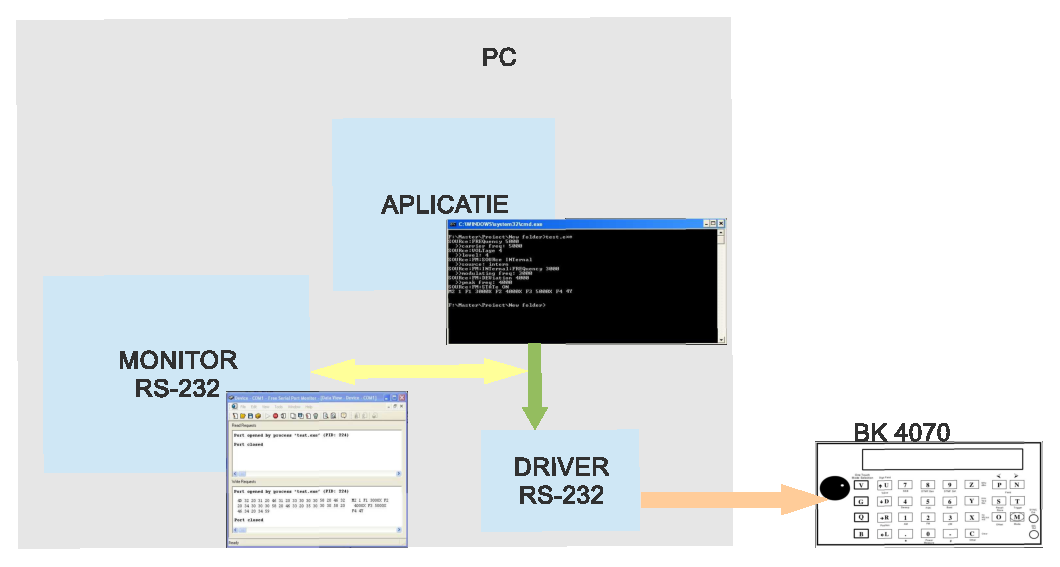
\epsfig{file=Figuri/sistem_.eps,width=1.1\linewidth,clip=}
  \caption{Sistemul implementat}
  \label{figsistem}
\end{figure}
